\documentclass[11pt,a4paper]{article}
\usepackage{fontspec}
\setmainfont{TeX Gyre Pagella}
\newfontfamily\headfont{Inter}[UprightFont=*-ExtraBold,BoldFont=*-ExtraBold,Extension=.otf,Path=/usr/share/fonts/opentype/inter/]
\usepackage[a4paper,margin=2.3cm]{geometry}
\usepackage{graphicx,booktabs,float,caption,array,xcolor,longtable}
\usepackage{xurl}
\usepackage[hidelinks]{hyperref}
\usepackage{titlesec}
\usepackage[round]{natbib}
\usepackage{setspace}
\setstretch{1.05}
\renewcommand{\topfraction}{0.9}
\renewcommand{\bottomfraction}{0.8}
\renewcommand{\textfraction}{0.1}
\renewcommand{\floatpagefraction}{0.75}
\setlength{\parindent}{0pt}
\setlength{\parskip}{0.55em}
\titleformat{\section}{\headfont\Large}{\thesection}{0.8em}{}
\titleformat{\subsection}{\headfont\large}{\thesubsection}{0.8em}{}
\captionsetup{font=small,labelfont=bf}
\urlstyle{same}
\hypersetup{pdftitle={Where the Asylums Were},pdfauthor={Tristan Hotham}}

\begin{document}
\begin{center}
{\Large\bfseries Where the Asylums Were\par}
\vspace{0.4em}
{\large Britain's county asylums and psychiatric hospitals, from the 1808 Act to Care in the Community:\\244 places in English Wikipedia\par}
\vspace{1.2em}
{\large Tristan Hotham\par}
\vspace{0.3em}
{\small Independent researcher\\
ORCID: 0000-0003-4931-9349\\
DOI: https://doi.org/10.5281/zenodo.23873001\par}
\vspace{0.8em}
2026
\end{center}

\begin{quote}
\small
\begin{center}\textbf{Abstract}\end{center}
I build an open dataset of Britain's lunatic asylums and later psychiatric hospitals from English Wikipedia and use it to describe when they opened, how large they became, when they closed and what their sites are now. Of 659 articles found by walking Wikipedia's psychiatric and defunct hospital categories, 244 describe a single asylum, psychiatric hospital or institution for people with learning disabilities; 233 can be located. Openings came in two waves, peaking in the 1860s (30) after the Lunacy and County Asylums Acts of 1845 and again in the 1900s (26); 62\% of places with an opening year opened between 1845 and 1914. The number open rose to 199 and stayed close to that level from the 1950s to the early 1980s. Closures were concentrated after Enoch Powell's Water Tower speech of 1961, but late: 64\% of the 155 dated closures fell between 1980 and 1999, 83 in the 1990s alone. The median Victorian asylum lasted 126 years. The largest stated size is Whittingham's 3,533 patients in 1939. London's asylums formed a ring: 28 opened between 1830 and 1939 lie 10 to 40 km from Charing Cross against 7 within 10 km, including the five hospitals of the Epsom cluster, all within 2.1 km of each other. Of 173 places no longer open, 47\% are now homes, 10\% have another use and 13\% are recorded as demolished; for 30\% the articles do not say. 34\% of the articles report a listed building. The dataset is uneven and incomplete, and I document its selection rules and limits.

\textbf{Keywords:} asylums; psychiatric hospitals; history of psychiatry; deinstitutionalisation; Care in the Community; Lunacy Act 1845; historic buildings; Wikipedia; open data; mapping
\end{quote}

\section{Introduction}
For most of the nineteenth and twentieth centuries the main public provision in Britain for people with a mental illness or a learning disability was the asylum: a large institution, usually built by a county or borough, standing in its own grounds outside a town. The County Asylums Act 1808 allowed counties in England and Wales to build them; the Lunacy Act and County Asylums Act of 1845 made the network general and set up the Lunacy Commission \citep{wiki1808,wiki1845}. The Mental Treatment Act 1930 renamed them mental hospitals \citep{wiki1930}; the Mental Health Act 1959 aimed to move care into the community \citep{wiki1959}; and in 1961 the Minister of Health, Enoch Powell, described them as ``isolated, majestic, imperious'' and predicted their end \citep{wikipowell}. The National Health Service and Community Care Act 1990 completed the policy known as Care in the Community \citep{wikicc}.

There is a large literature on this history, and enthusiasts have documented many individual sites. This paper asks what an open, reproducible source can show at the scale of the whole system. English Wikipedia has articles on several hundred British hospitals with infoboxes giving opening and closing years, coordinates and sometimes bed numbers, and leads that often say what became of the site. I turn these into a dataset, map it (\url{https://maps.tristanhotham.com/asylums/}), and report the rise and fall of the asylum in numbers, with the limits that such a source imposes. The study is a companion to an earlier one on the traces of the workhouse.

A note on language: I use the historical names of institutions (``lunatic asylum'', ``mental deficiency colony'') because they are part of the record; they are not terms for people.

\section{Data}
\textbf{Articles.} The articles were found by walking 22 Wikipedia categories under Psychiatric hospitals in the United Kingdom, Former psychiatric hospitals in the United Kingdom and Defunct hospitals in England, Scotland and Wales, three levels deep, in 2026. For each of the 659 articles I have its revision id, categories, Wikidata id, the API's coordinates where the API returned them (138 articles) and the first 6,000 characters of its wikitext, which usually covers the infobox and the lead. Context articles on the Acts, on Powell, on Care in the Community and on several asylums supply the history quoted in the text \citep{wiki1774,wiki1808,wiki1845,wiki1930,wiki1959,wikipowell,wikicc,wikiepsom,wikiwhit,wikicolney,wikibethlem,wikila}.

\textbf{Wikidata.} I was also given a Wikidata extract of UK items that are instances of subclasses of item Q1774898. That item is the class for clinics, not psychiatric hospitals, and none of the extract's 213 items matches an article in the Wikipedia set (157 are community health centres; most others are clinics and dental practices). I report this and do not use it.

\textbf{Geography.} Coastlines and towns are from Natural Earth \citep{naturalearth}; county outlines from the ONS and OSNI.

\section{Methods}
\subsection{Which articles count}
An article is kept if it describes a single place and (A) the first two sentences of its lead call it a psychiatric or mental hospital, an asylum, a lunatic asylum or an institution for people with learning disabilities, using any of the words psychiatric, asylum, lunatic, mental, insane, madhouse, idiot, imbecile, feeble-minded, learning or intellectual disability, epileptic or psychogeriatric (``Metropolitan Asylums Board'', ``sick asylum'', ``orphan asylum'' and ``asylum seeker'' excluded); or (B) its infobox type or speciality uses one of these words and does not say general, teaching or district; or (C) Wikipedia files it in a psychiatric hospital category and one of the words appears in its text. 225 articles pass test A, and 190 pass all three. Articles about people, NHS trusts, tribunals, charities, units ``based at'' another hospital, the Epsom Cluster as a group and a drug and alcohol rehabilitation centre are dropped, as is one general hospital checked by hand; one pair of articles describing the same site is merged. Table~\ref{tab:select} gives the counts.

\begin{table}[tbp]\centering\small\caption{From Wikipedia articles to places.}\label{tab:select}\begin{tabular}{lr}\toprule Step & Articles\\\midrule
Articles found & 659\\
General and other hospitals (dropped) & 355\\
Not hospital articles (dropped) & 45\\
People, organisations, units and group articles (dropped) & 14\\
Duplicate of the same site (merged) & 1\\
Places kept & 244\\
of which located & 233\\
of which with an opening year & 230\\
of which with a closing year & 155\\
of which with a stated size & 96\\
of which still open & 71\\
\bottomrule\end{tabular}\end{table}

\subsection{Fields}
Coordinates come from the coord template in the wikitext (231) or the API (2). The opening year is the first year in the infobox field founded, opened or constructed; failing that, a year attached to ``opened'', ``established'' or ``founded'' in the lead, then to ``the hospital opened'' in the text, then a ``NNNN establishments'' category. The closing year comes the same way from the closed field, the lead, ``the hospital closed'' in the text, and ``Hospitals disestablished in NNNN''. A lead in the present tense (``is a psychiatric hospital'') with no closing year marks a place as still open, and outranks a closing year found only in the text. Size is the infobox beds figure or, if larger, the largest number of beds, patients, inmates or residents the text states after a word of capacity (accommodate, house, hold, designed for, had, peak); counts of deaths, transfers or admissions are excluded. These are capacities at different dates, not a common measure. Opening and closing years are given for 230 and 155 places.

\subsection{What the site is now}
The fate of each site is read from keywords in its lead or, if the lead says nothing, in the rest of the opening text. Homes: flats, apartments, housing, residential use or development, with a verb of conversion or redevelopment in the same clause, and not plans or proposals. Other use: a college, university, campus, offices, hotel, prison, museum and so on. Demolished: demolished, razed, pulled down, with no new use stated. Derelict: derelict, disused, in ruins, left empty. Still a hospital: open, as above. The order of precedence is still a hospital, homes, other, derelict, demolished, so a cleared site rebuilt as housing counts as homes. Listed status is read from phrases such as ``Grade II listed'' or ``Category B listed'' and from listed building categories.

\subsection{Geography}
Each located place is assigned to a county by point in polygon. Distance to the nearest town is the great circle distance to the nearest of 41 Natural Earth places in the UK, Ireland and the Isle of Man with a present-day population of at least 100,000. The London ring is the band 10 to 40 km from Charing Cross.

\section{Results}
\subsection{Coverage}
The 244 places are 171 located in England, 42 in Scotland, 14 in Wales, 5 in Northern Ireland and 1 on the Isle of Man, with 11 unlocated (Figure~\ref{fig:map}). They include 14 institutions for people with learning disabilities, 9 secure hospitals and a number of modern mental health units, some on the sites of old asylums.

\begin{figure}[tbp]\centering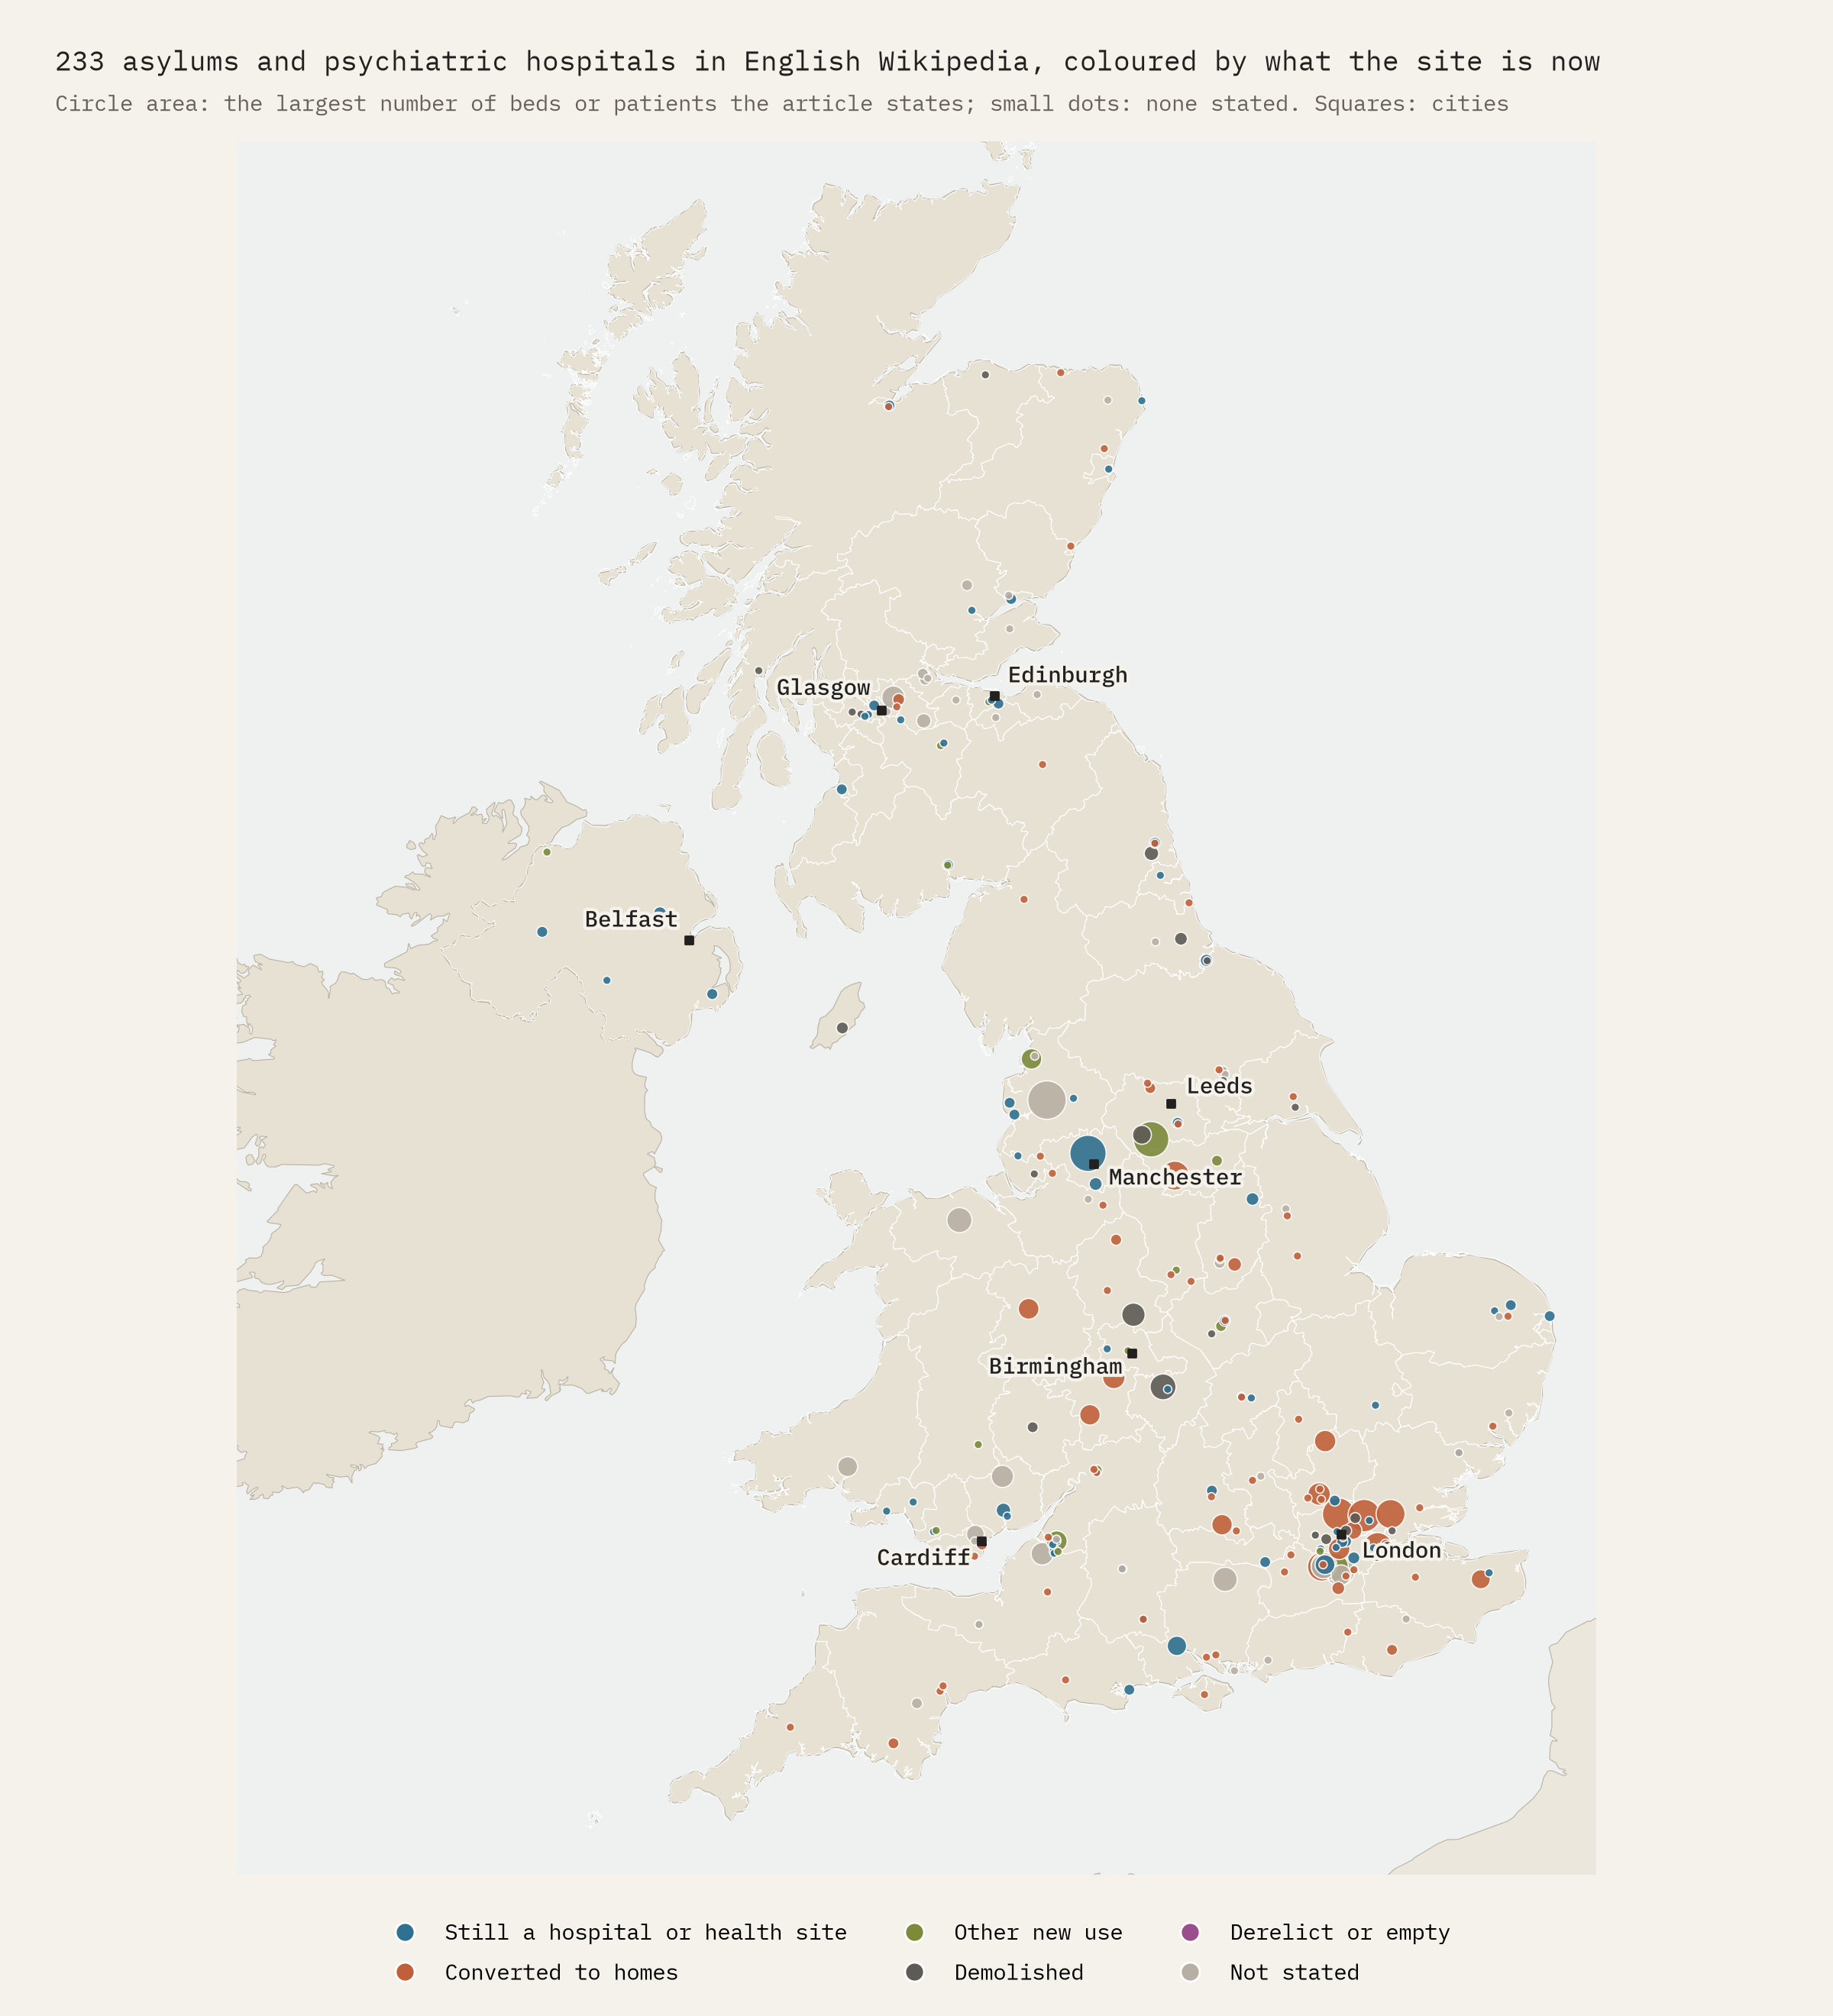
\includegraphics[width=.92\textwidth]{f_map.png}
\caption{Asylums and psychiatric hospitals in the data, coloured by what the site is now and sized by the largest stated beds or patients.}\label{fig:map}\end{figure}

\subsection{Two waves of building}
Nine places opened before 1800, from Bethlem (founded 1247) to the charitable and private asylums of the eighteenth century. Under the permissive Act of 1808, 31 opened between 1808 and 1844. After 1845 the pace rose to a peak of 30 openings in the 1860s and 24 in the 1870s, fell to 10 in the 1880s and rose again to 19 in the 1890s and 26 in the 1900s (Figure~\ref{fig:dec}). After 1914 few new asylums opened: 22 between 1915 and 1947, 9 between 1948 and 1989 and 15 since 1990, the last mostly small units. The median opening year is 1874.

\begin{figure}[tbp]\centering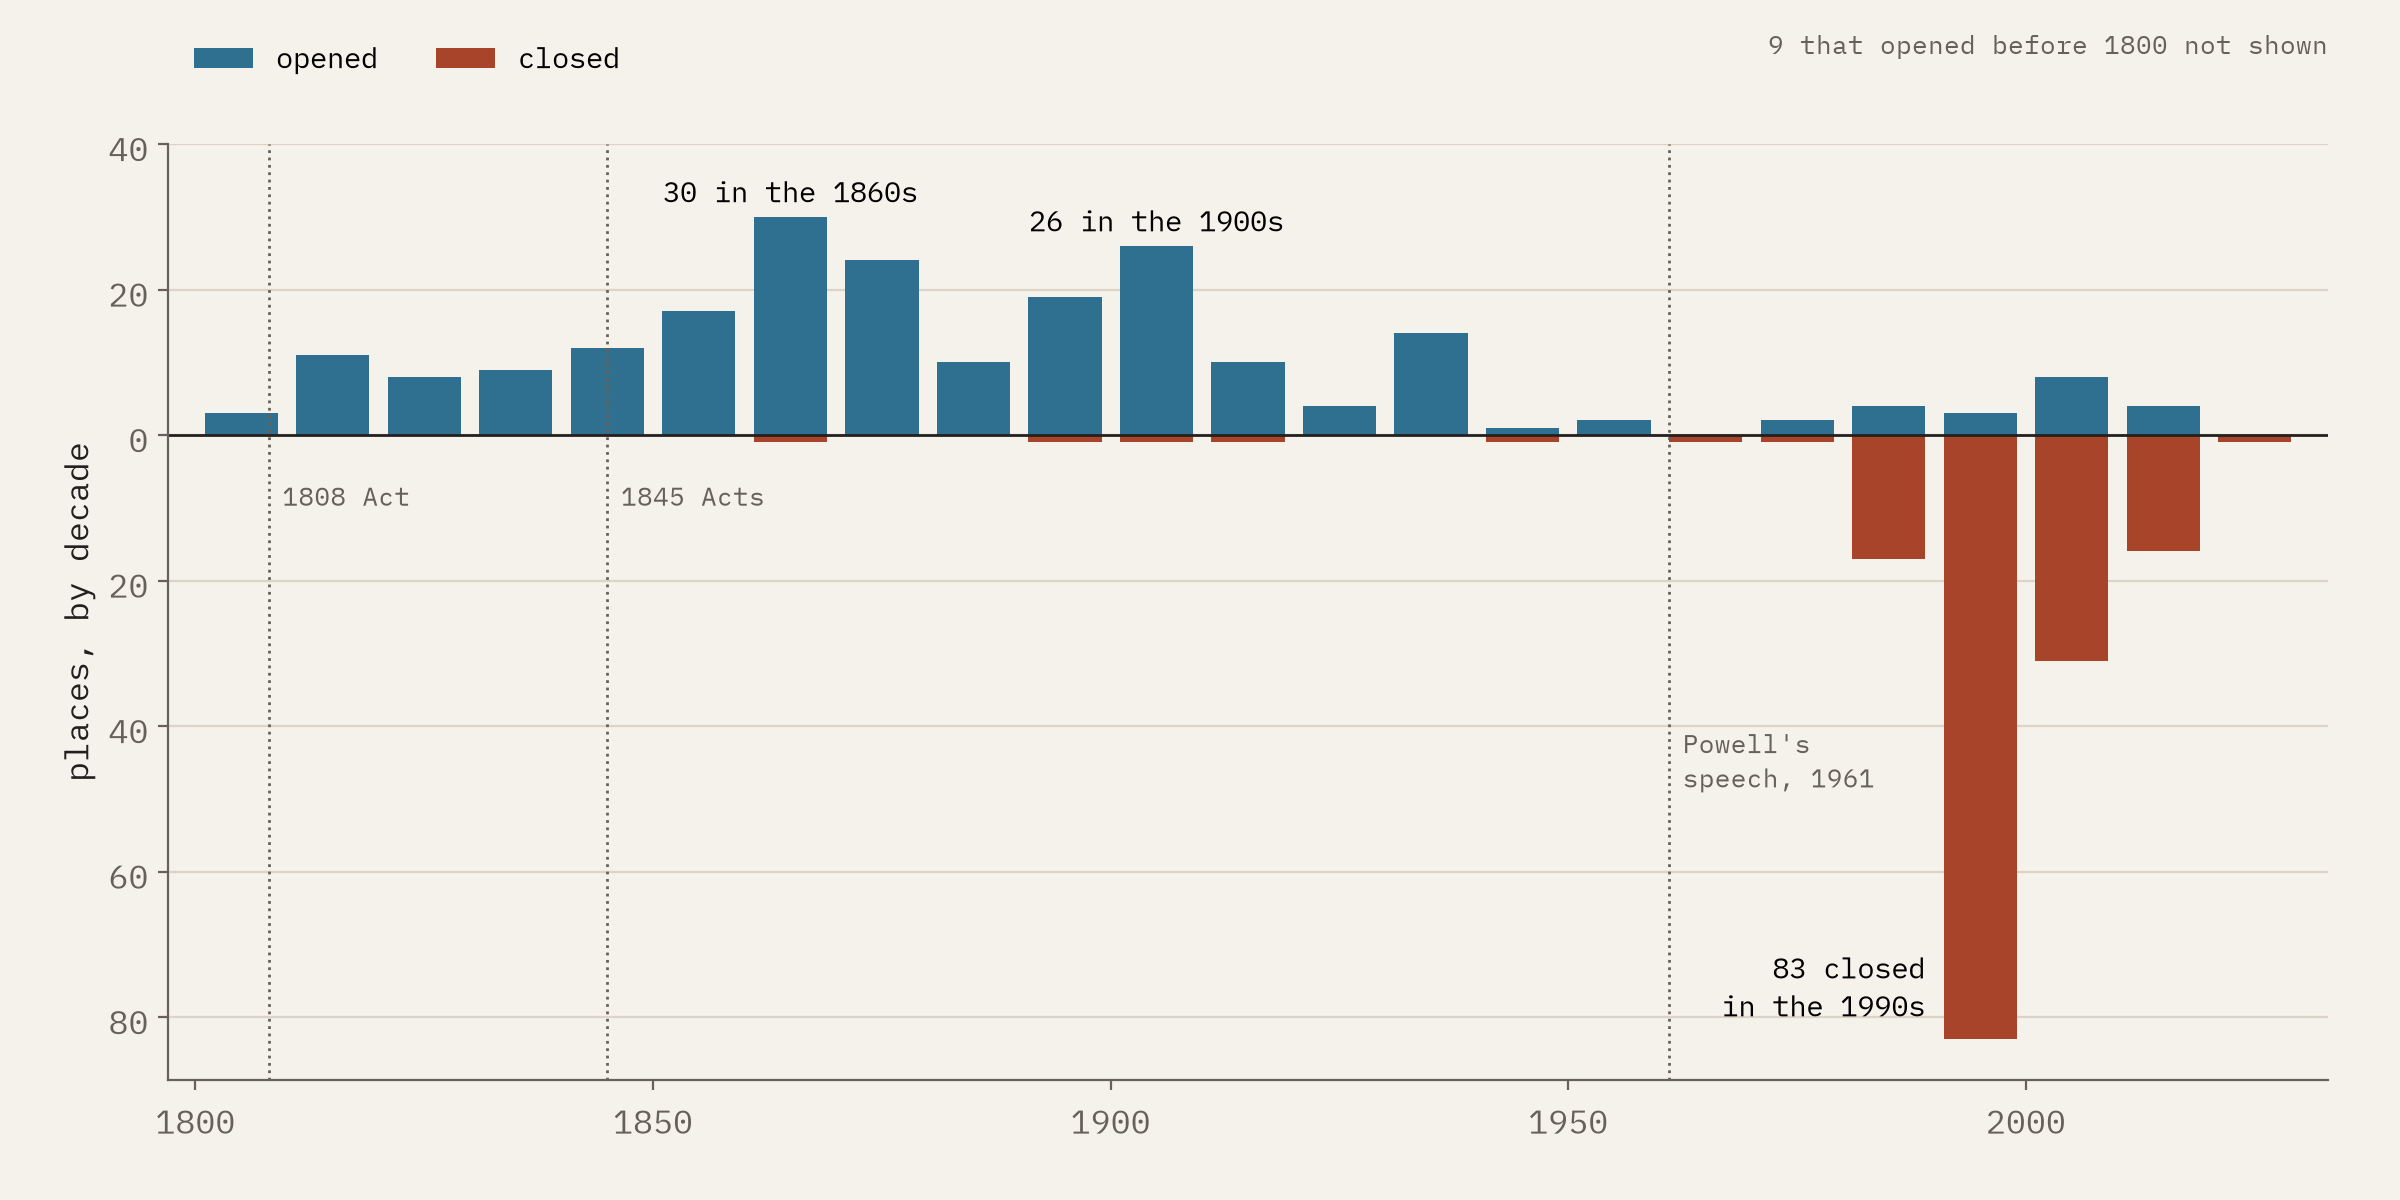
\includegraphics[width=\textwidth]{f_decades.png}
\caption{Openings (up) and closures (down) by decade.}\label{fig:dec}\end{figure}

\subsection{A long plateau and a late fall}
The number open (Figure~\ref{fig:open}) rose from 43 in 1845 to 145 in 1900 and 175 in 1914, and reached 199, a level held from 1972 to 1983. Of the 155 closures with a year, 5 came before 1961 and 2 between 1961 and 1979; 17 came in the 1980s, 83 in the 1990s, 31 in the 2000s and 16 in the 2010s. Of the 198 places open in 1961, 149 (75\%) have closed, with a median closing year of 1996. The policy announced in 1961 therefore took effect mostly two to four decades later. For the 131 asylums opened between 1808 and 1914 with both years, the median life was 126 years and 78\% lasted a century or more.

\begin{figure}[tbp]\centering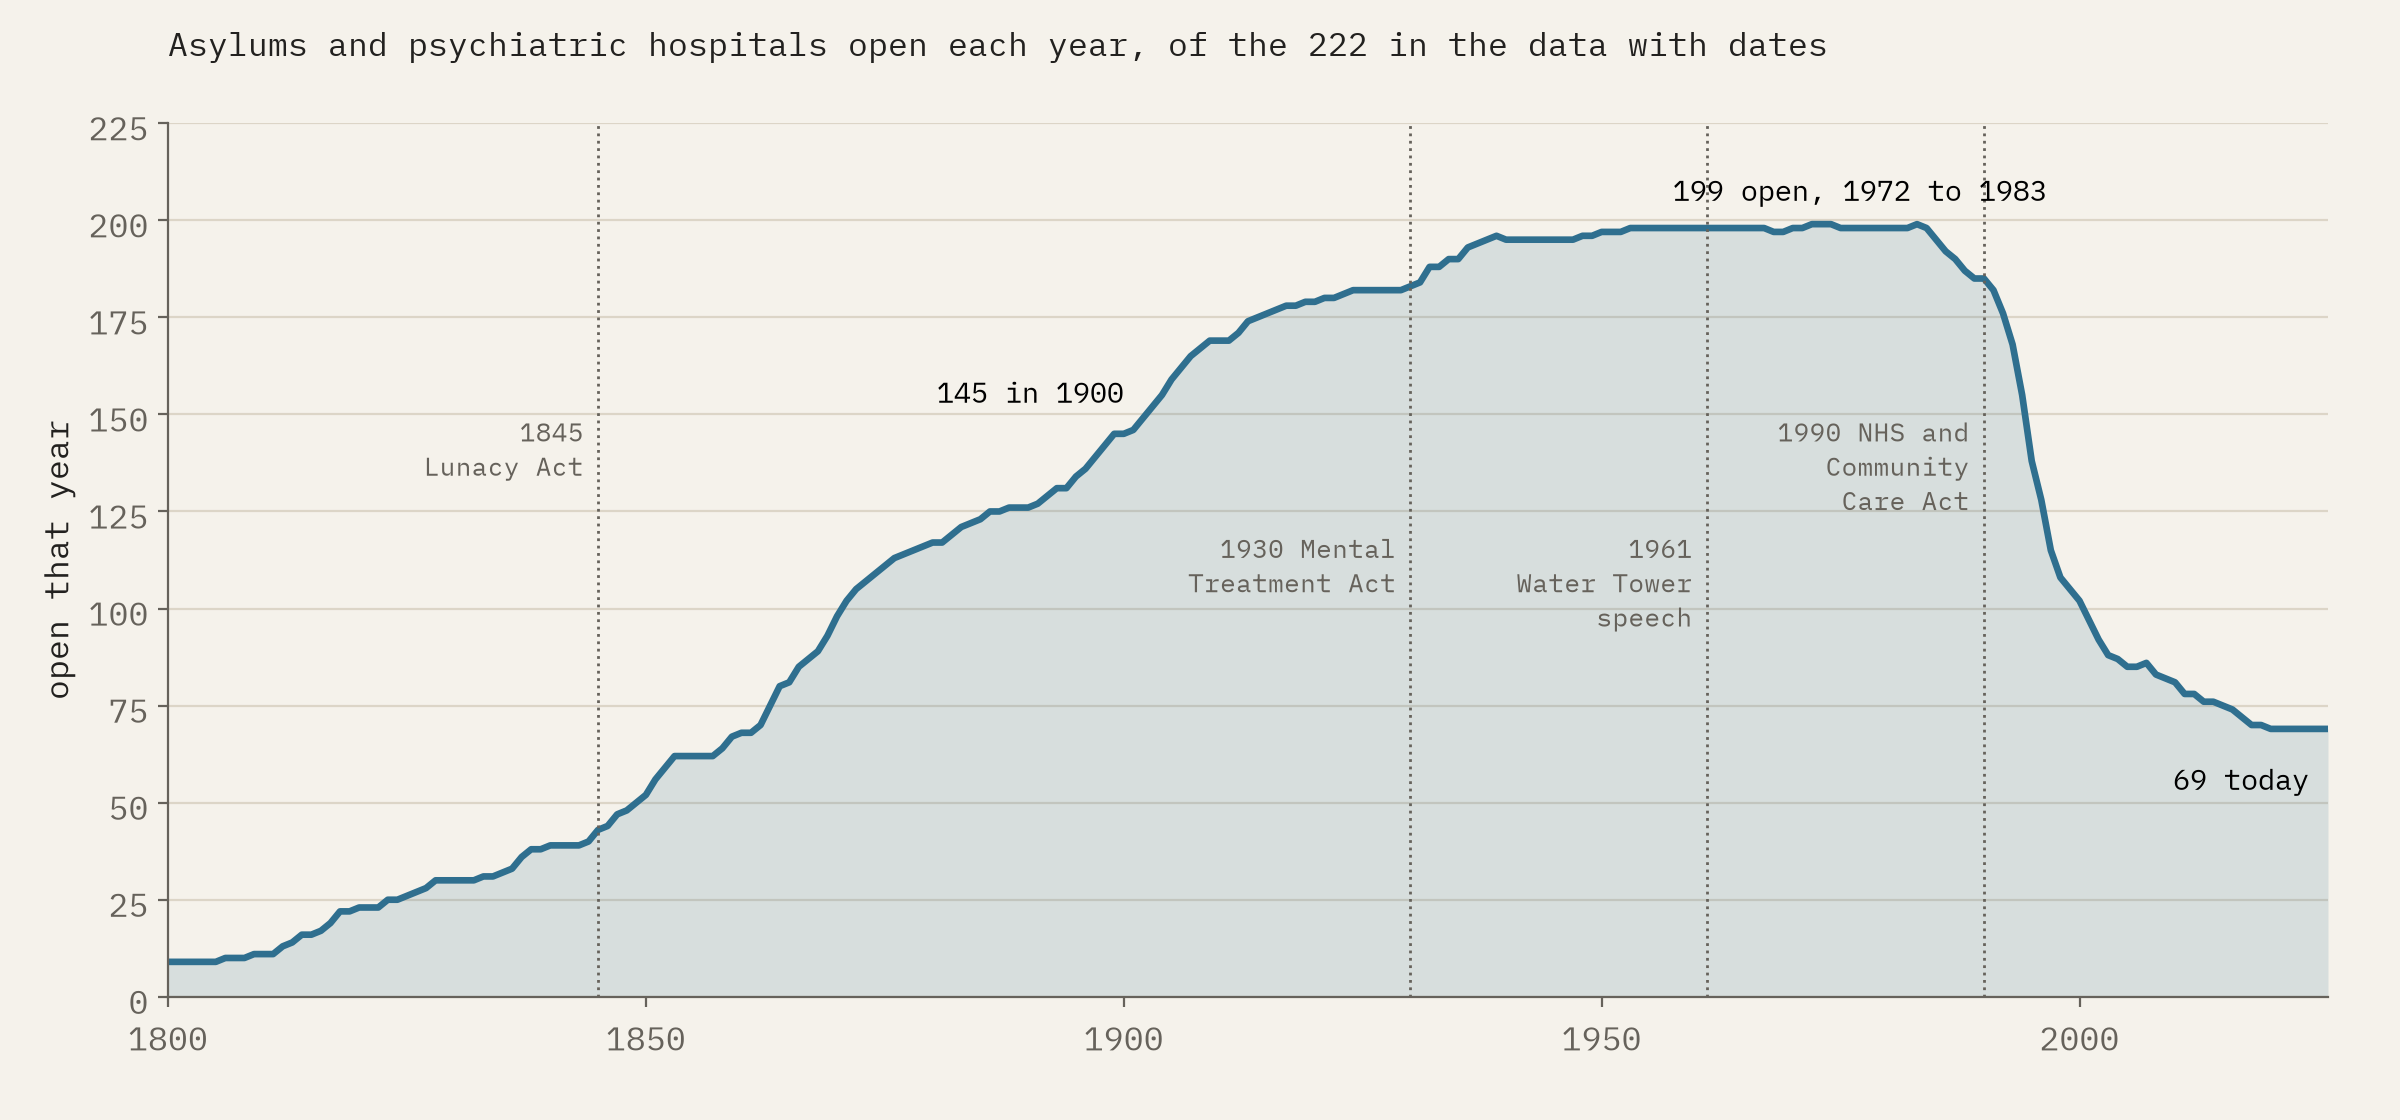
\includegraphics[width=\textwidth]{f_open.png}
\caption{Places open in each year, of the 222 with an opening year and either a closing year or no recorded closure.}\label{fig:open}\end{figure}

\subsection{Size}
96 places state a size (34 from the infobox, 62 from the text). 30 held 1,000 or more at some date and 10 2,000 or more (Table~\ref{tab:big}, Figure~\ref{fig:big}). Whittingham in Lancashire, with 3,533 patients in 1939, is described in its article as the largest mental hospital in Great Britain \citep{wikiwhit}. The median stated size of asylums opened 1808 to 1914 is 500, against 122 for units opened since 1990.

\begin{table}[tbp]\centering\footnotesize\caption{The fifteen largest stated sizes (beds or patients at some date), with source.}\label{tab:big}\begin{tabular}{llrrrl}\toprule Place & County & Opened & Closed & Size & Source\\\midrule
Whittingham Hospital & Lancashire & 1873 & 1995 & 3,533 & infobox\\
Prestwich Hospital & Greater Manchester & 1851 &  & 3,135 & text\\
Storthes Hall Hospital & West Yorkshire & 1904 & 1992 & 3,000 & text\\
Friern Hospital & Greater London & 1849 & 1993 & 2,500 & text\\
Claybury Hospital & Greater London & 1893 & 1997 & 2,500 & infobox\\
Middlewood Hospital & South Yorkshire & 1872 & 1996 & 2,000 & text\\
Bexley Hospital & Kent & 1898 & 2001 & 2,000 & text\\
Cane Hill Hospital & Greater London & 1882 & 2008 & 2,000 & text\\
Warley Hospital & Essex & 1853 & 2001 & 2,000 & text\\
West Park Hospital, Epsom & Surrey & 1921 & 2003 & 2,000 & text\\
Banstead Hospital & Surrey & 1877 & 1986 & 1,700 & text\\
Central Hospital, Hatton & Warwickshire & 1852 & 1995 & 1,600 & text\\
Horton Hospital & Surrey & 1902 & 1997 & 1,587 & text\\
North Wales Hospital & Clwyd & 1844 & 1995 & 1,500 & infobox\\
Manor Hospital, Epsom & Surrey & 1899 & 1996 & 1,417 & text\\
\bottomrule\end{tabular}\end{table}

\begin{figure}[tbp]\centering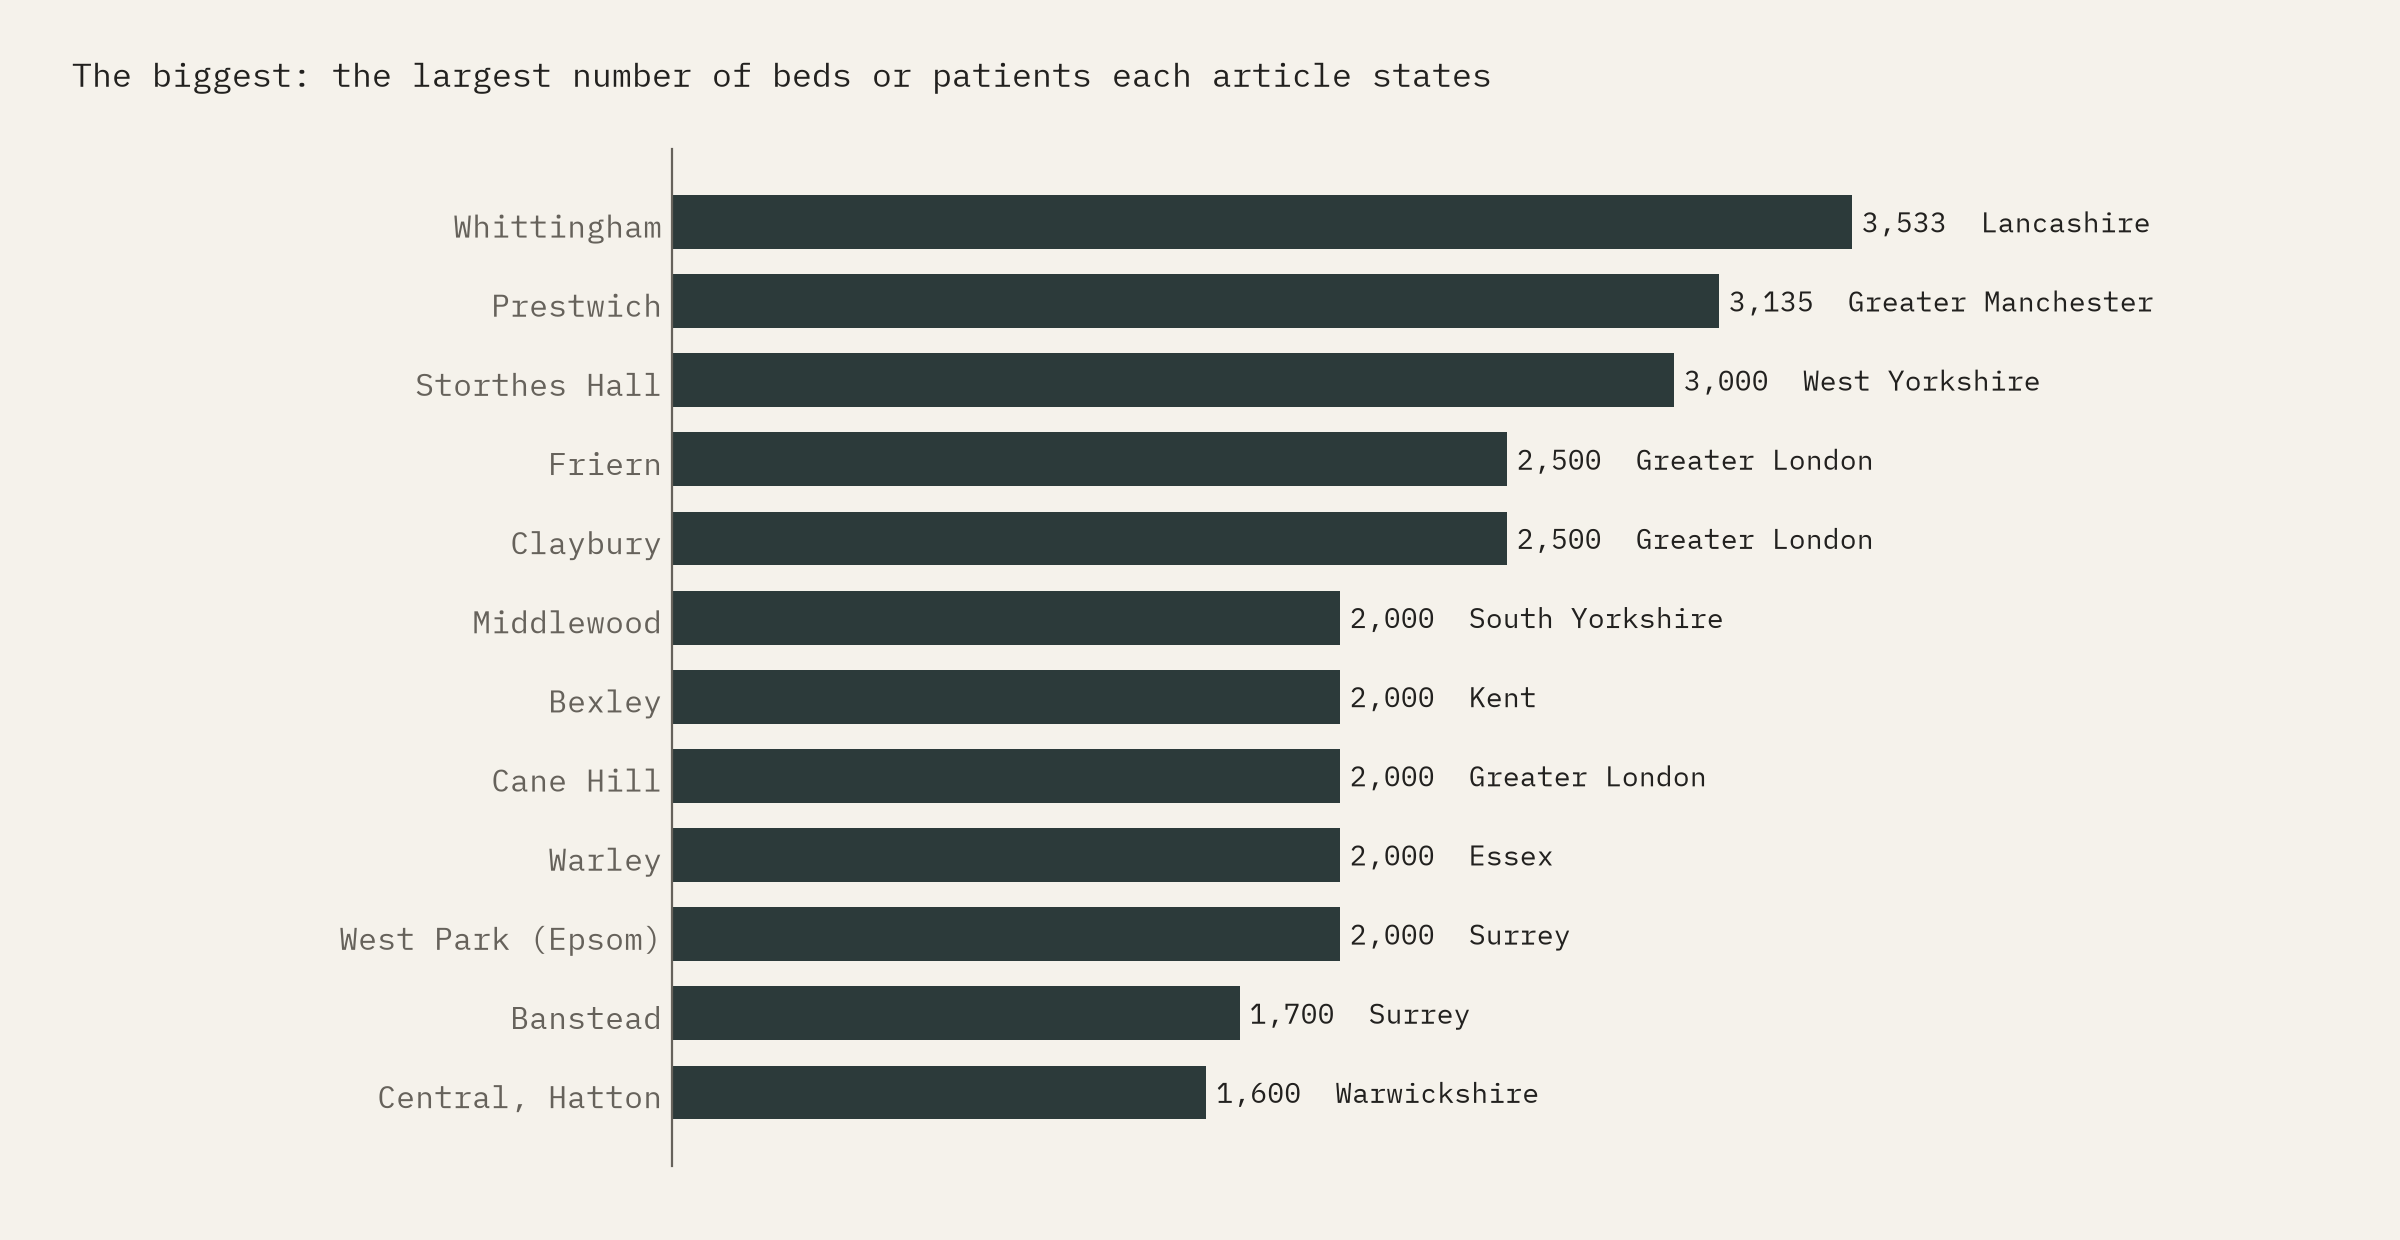
\includegraphics[width=\textwidth]{f_biggest.png}
\caption{The twelve largest stated sizes.}\label{fig:big}\end{figure}

\subsection{Clusters and distance}
London placed its asylums in a ring outside the built-up area (Figure~\ref{fig:london}): of places opened 1830 to 1939, 7 lie within 10 km of Charing Cross and 28 between 10 and 40 km, a median 22.2 km out, 20 of them beyond today's Greater London boundary. The five Epsom hospitals, built by the London County Council on the Horton estate \citep{wikiepsom}, opened between 1899 and 1921 within 2.1 km of each other; four state sizes totalling 5,937. Across Britain, 88\% of asylums opened 1845 to 1914 are more than 5 km from the nearest town of 100,000 or more today (median 20.4 km), against 71\% of places opened since 1948 (Figure~\ref{fig:town}); present-day populations make this a rough measure.

\begin{figure}[tbp]\centering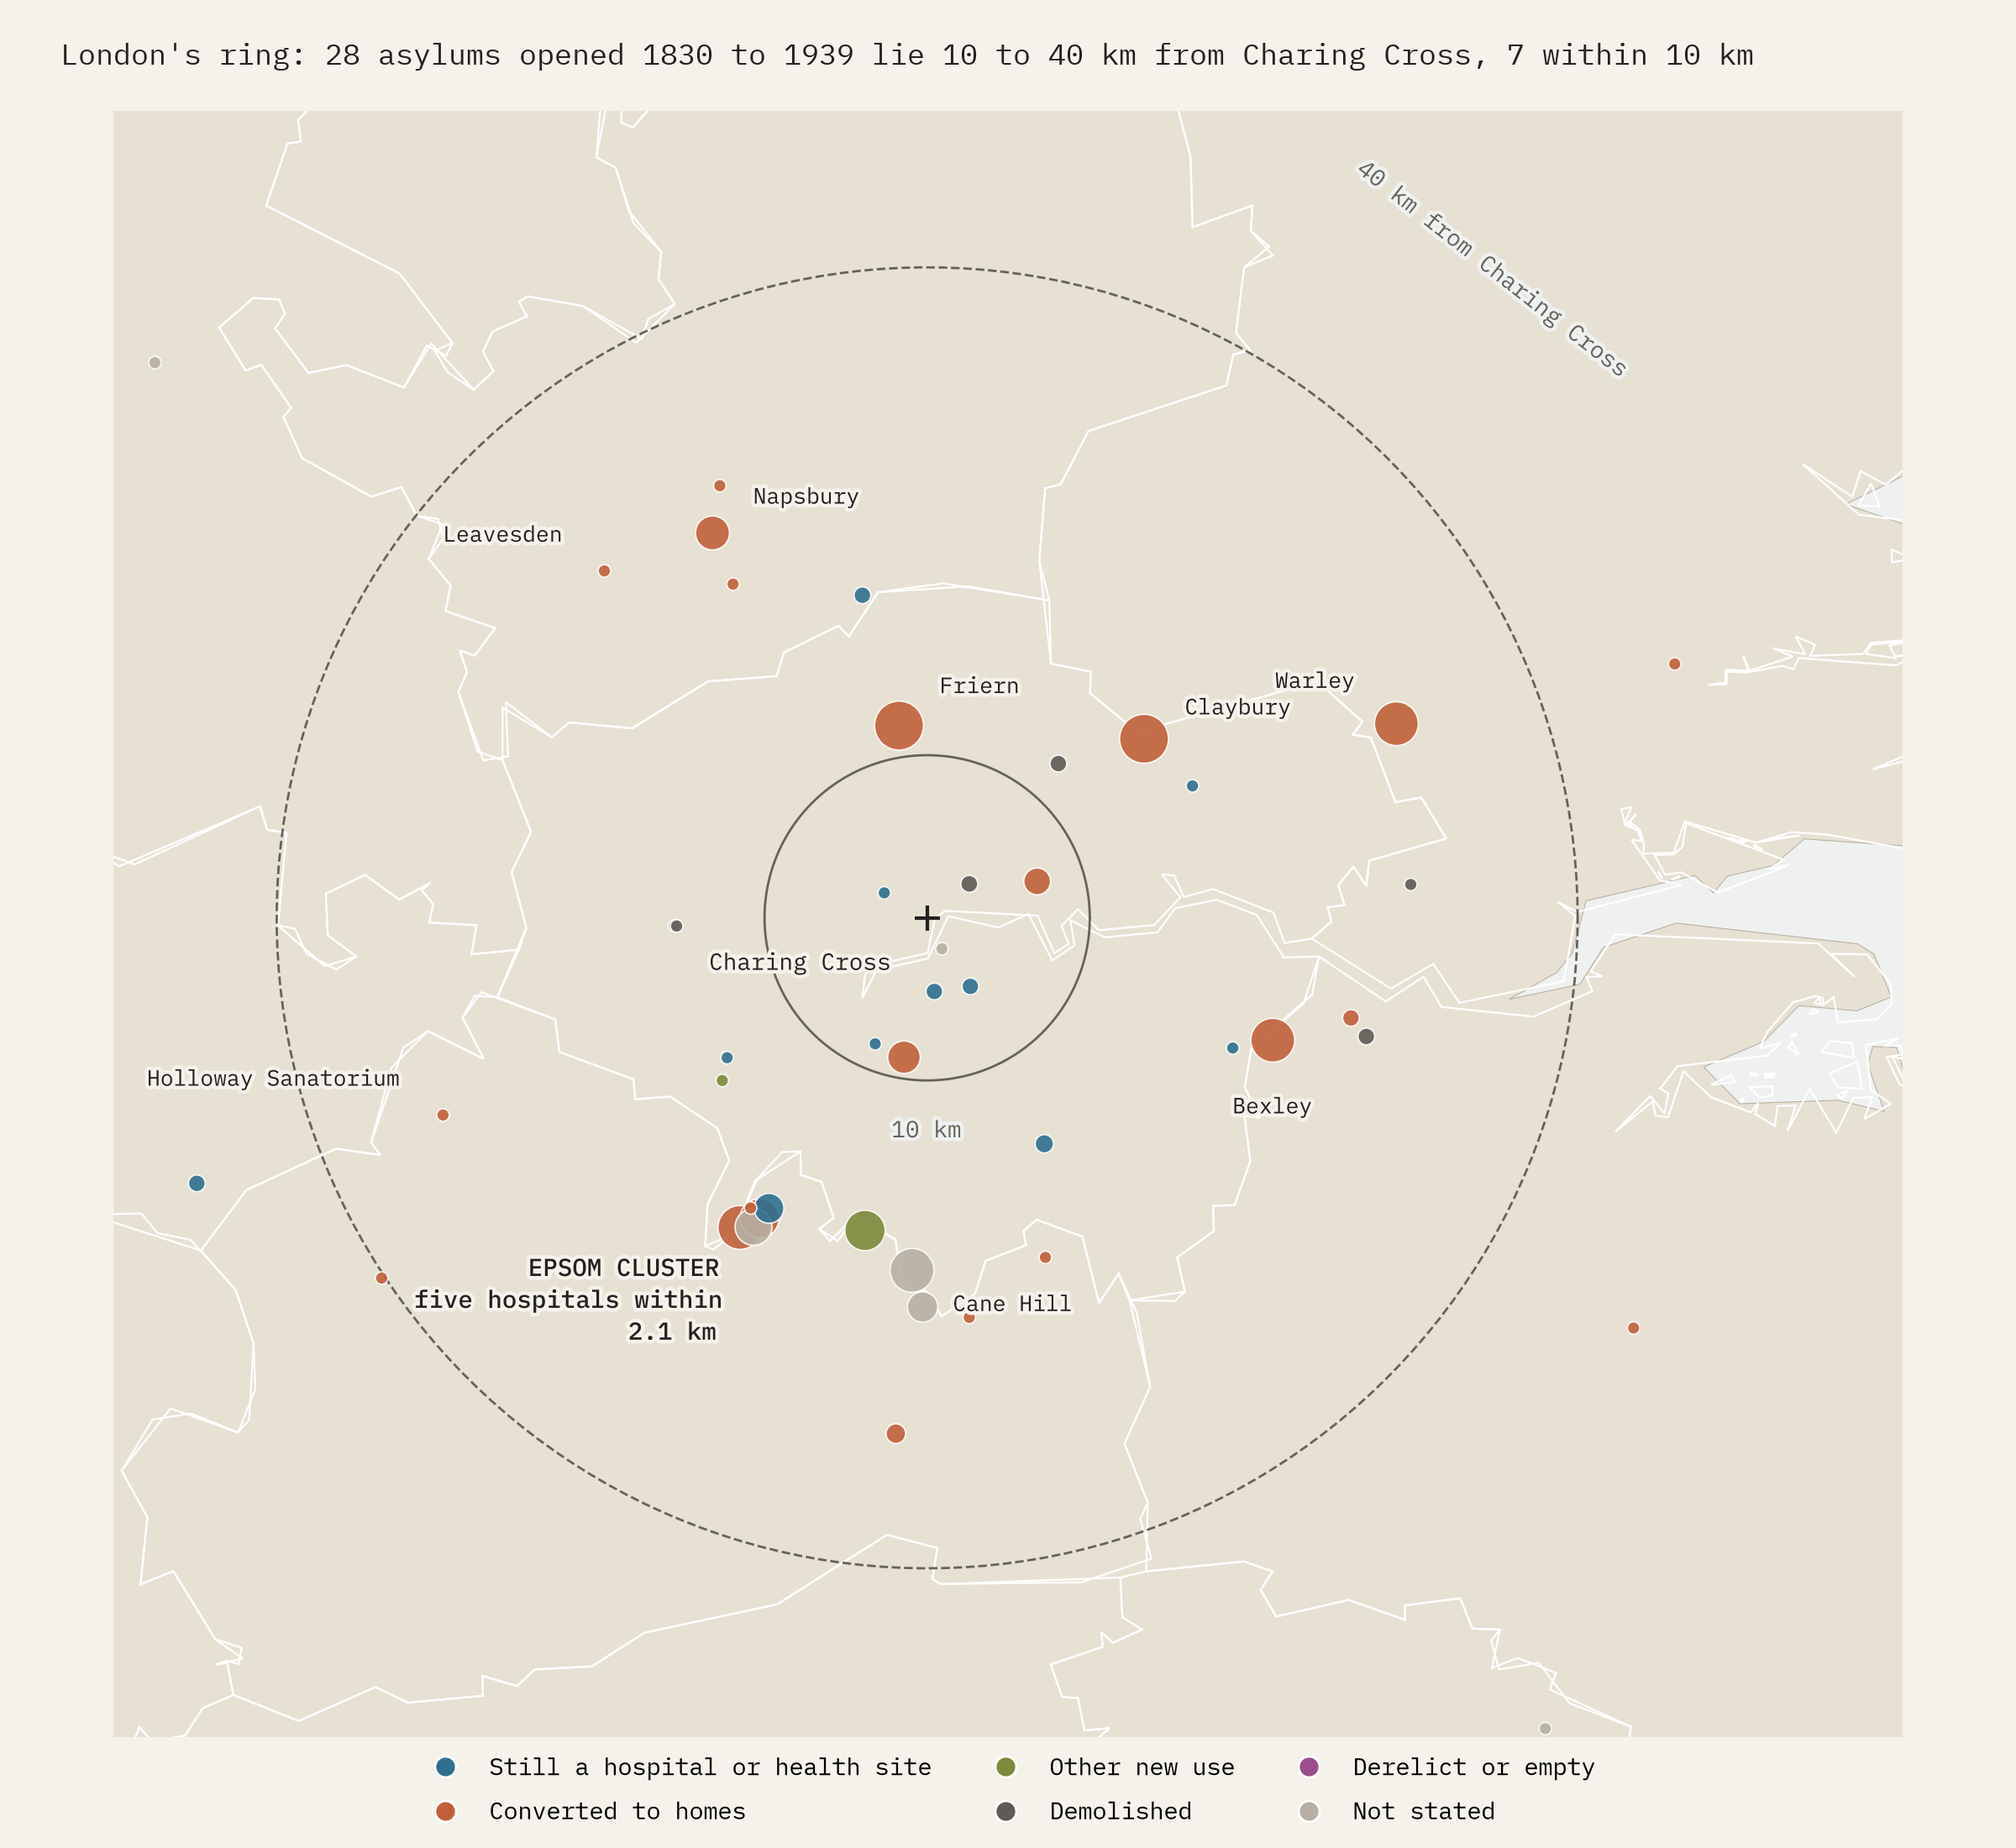
\includegraphics[width=.92\textwidth]{f_london.png}
\caption{The London ring: places within 40 km of Charing Cross, with the Epsom cluster.}\label{fig:london}\end{figure}

\begin{figure}[tbp]\centering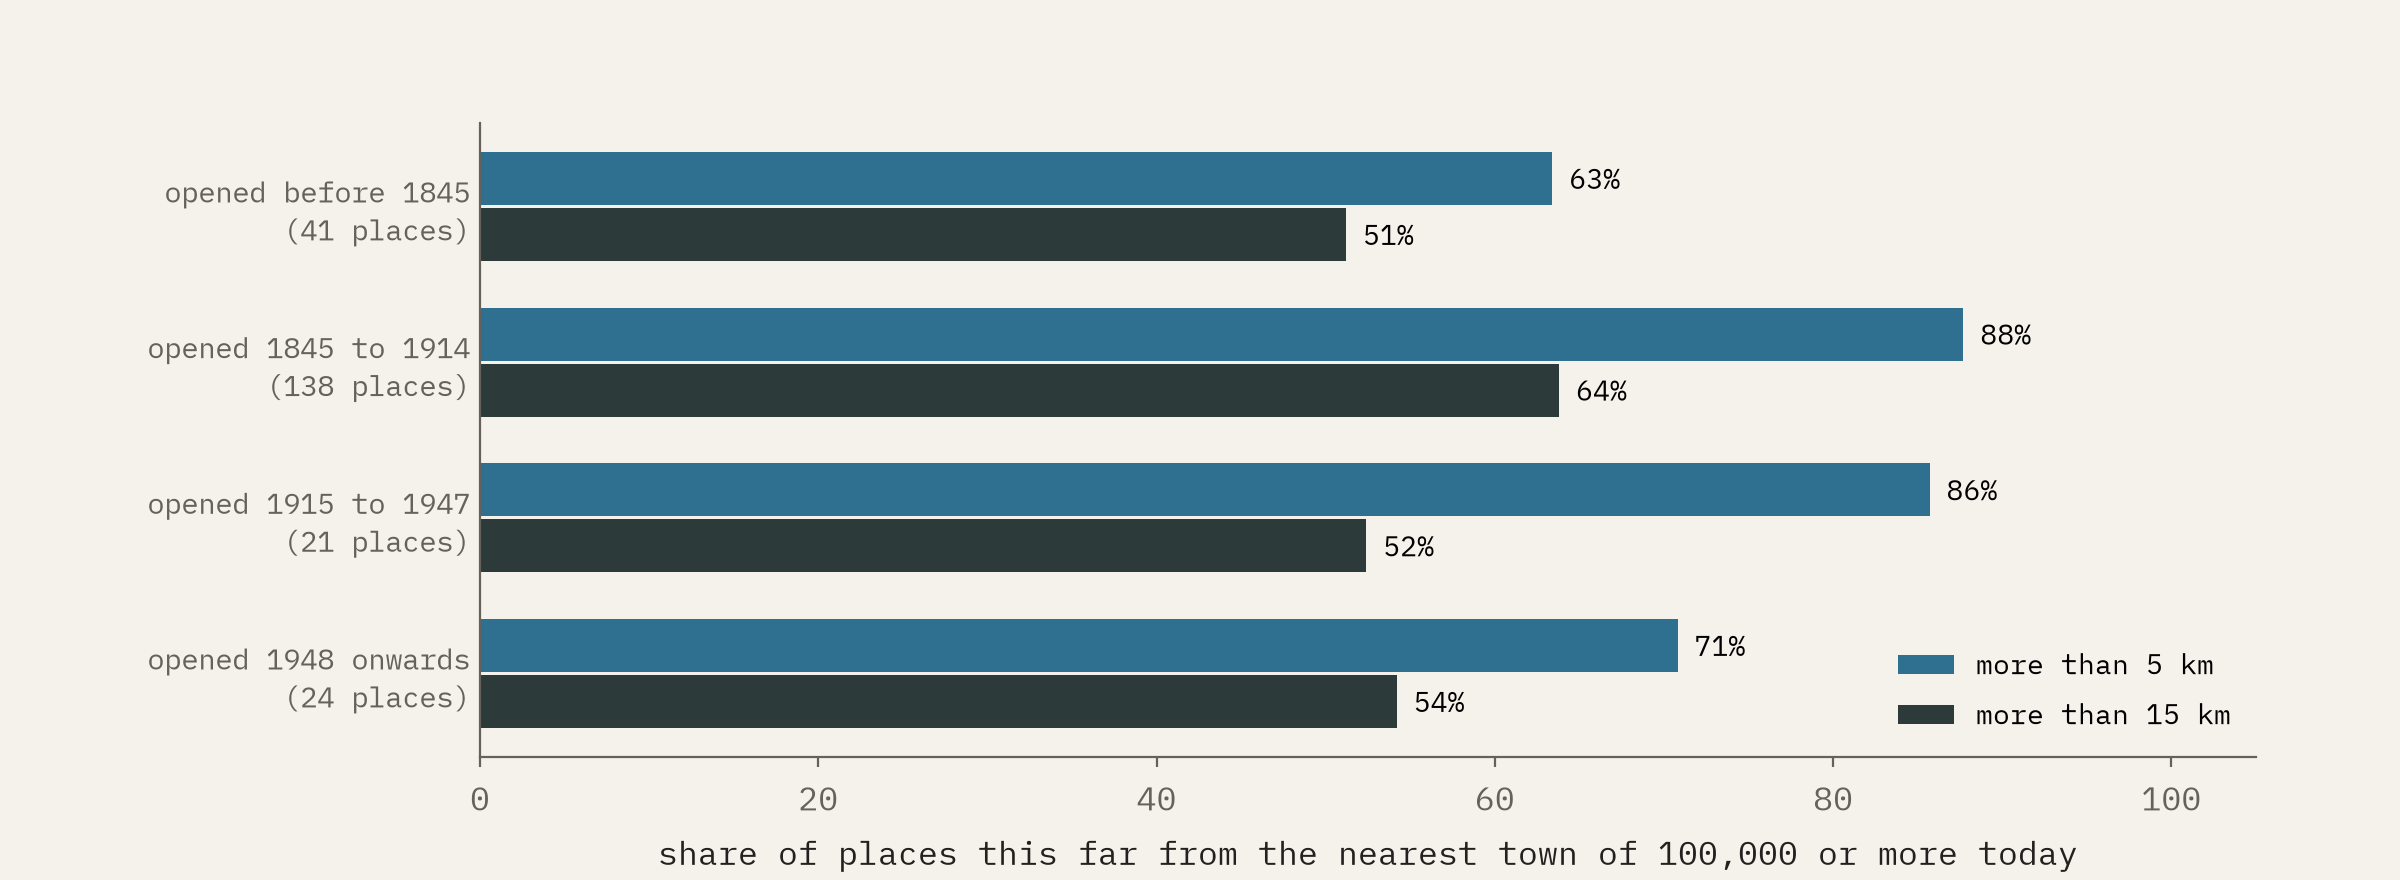
\includegraphics[width=\textwidth]{f_town.png}
\caption{Share of places more than 5 and 15 km from the nearest town of 100,000 or more today, by period of opening.}\label{fig:town}\end{figure}

\subsection{What the sites are now}
Of the 173 places no longer open, 81 (47\%) are now homes, 17 (10\%) have another use, 22 (13\%) are recorded as demolished with no new use stated and 2 as derelict; 51 (30\%) are not stated (Figure~\ref{fig:fates}). Among closed sites with a stated fate, 66\% are homes. 25 of the housing sites also mention demolition. The fate was found in the lead for 92 places and in the rest of the text for 101. 83 articles (34\%) report a listed building, 36\% of asylums opened 1808 to 1914 and 3 of 24 places opened since 1948; three are Grade I.

\begin{figure}[tbp]\centering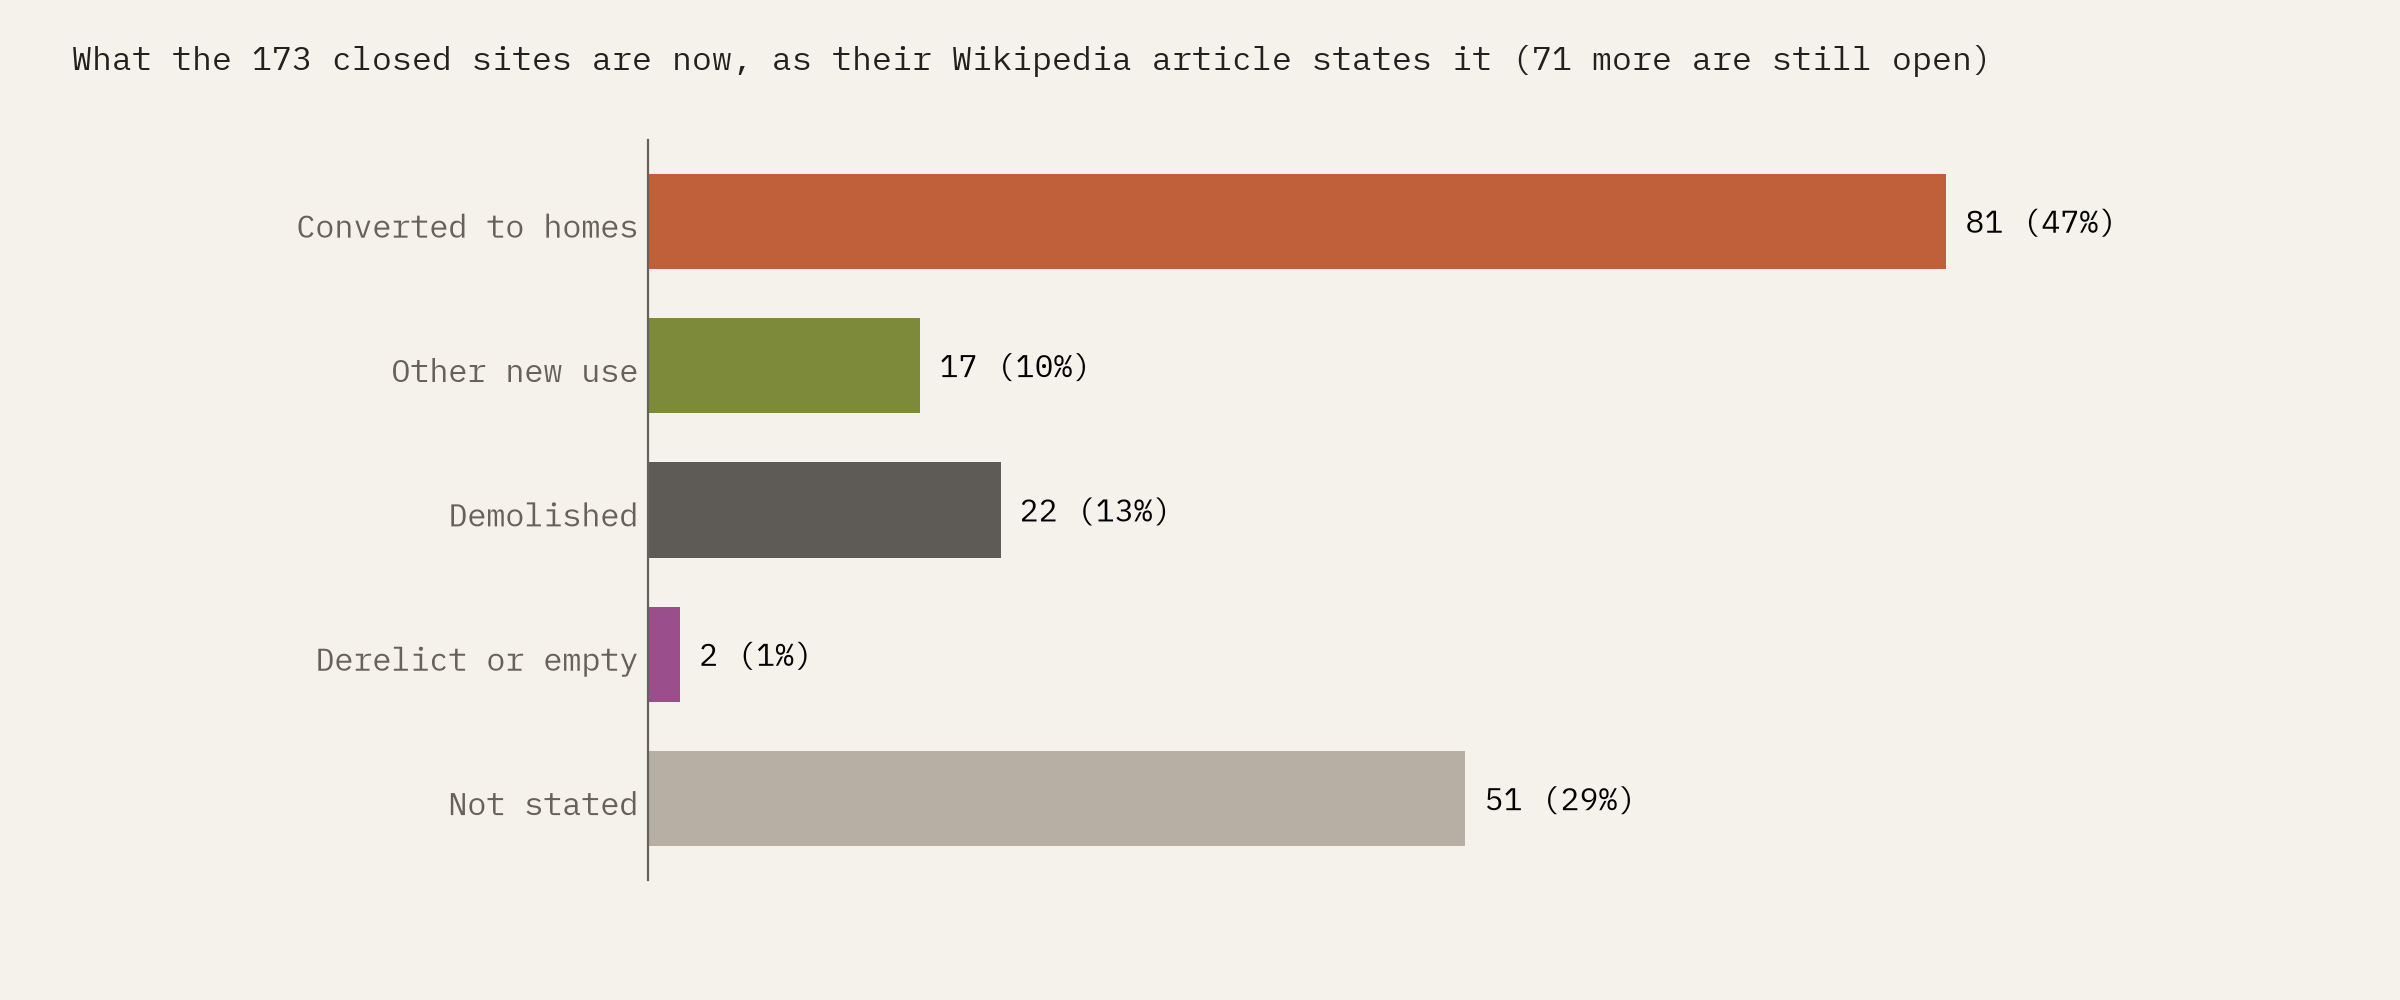
\includegraphics[width=\textwidth]{f_fates.png}
\caption{What the closed sites are now, as their articles state.}\label{fig:fates}\end{figure}

\subsection{Names}
141 articles (58\%) record a name with ``asylum'', 82 a ``mental hospital'' name and 73 both (Figure~\ref{fig:names}). Where a single year is given for a ``mental hospital'' name (33 places), 21 fall in 1920 to 1939, the period of the Mental Treatment Act 1930. 35 current titles begin with ``St''.

\begin{figure}[tbp]\centering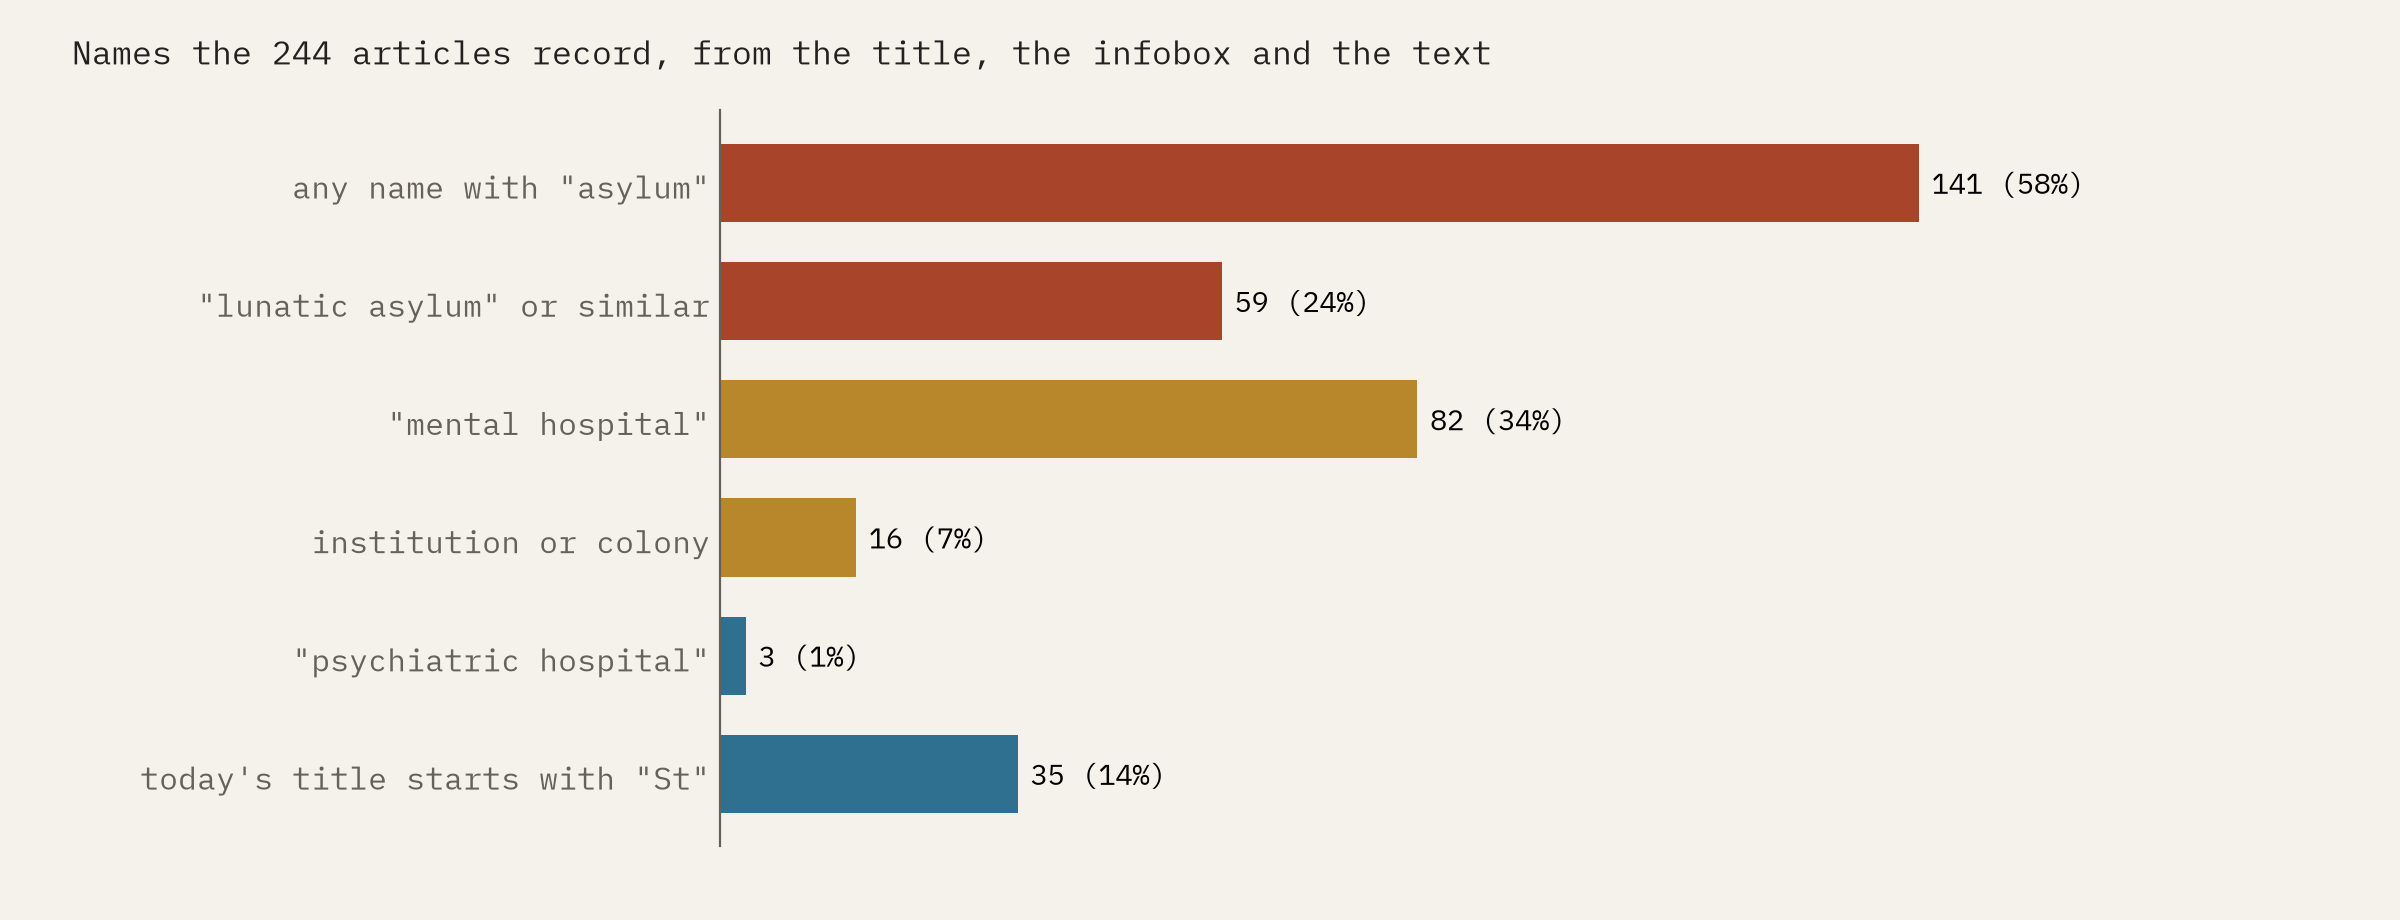
\includegraphics[width=\textwidth]{f_names.png}
\caption{Names recorded in the articles.}\label{fig:names}\end{figure}

\section{Limitations}
First, the data cover only places with a Wikipedia article in the categories walked; many asylums are missing, and Wales and Northern Ireland are thin. Second, the selection rules are keyword rules and include modern units and some private houses alongside the county asylums. Third, only the first 6,000 characters of each article were read, so later history, including fates, is often cut off. Fourth, years, sizes and fates are what the articles say, and the articles differ in what they count as opening, closing or capacity. Fifth, the fate rules can misread a sentence; every assignment is published with the phrase that triggered it so that it can be checked. Sixth, distances use present-day town populations.

\section{Conclusion}
Wikipedia, read with simple and published rules, recovers the shape of the asylum era in Britain: two waves of building after 1845 and around 1900, a long plateau through the middle of the twentieth century, and a concentrated closure in the 1980s and 1990s, a generation after Powell's speech. The buildings did not vanish. Most of the closed sites whose fate is recorded are now homes, often in the old wards, and a third of the articles report listed buildings. The asylums' successors are smaller and often on the same ground.

\section*{Data and code availability}
The interactive map is at \url{https://maps.tristanhotham.com/asylums/}. Data and code are at \url{https://github.com/Tristan-Hotham/asylums} and archived with this paper at https://doi.org/10.5281/zenodo.23873001. Code is released under the MIT licence, text and figures under CC BY 4.0, and the table derived from Wikipedia (data/asylums.csv) under CC BY-SA 4.0.

\section*{AI statement}
I wrote the text, with drafting and editing assistance from Claude (Anthropic), which also helped prepare the analysis code. I reviewed and checked all text and results.

\begin{thebibliography}{20}
\bibitem[Natural Earth(2026)]{naturalearth} Natural Earth (2026) Admin 0 countries and populated places, 1:10m. Public domain. \url{https://www.naturalearthdata.com/}
\bibitem[Wikipedia(2026a)]{wiki1774} Wikipedia contributors (2026) Madhouses Act 1774 (revision 1381750101). CC BY-SA 4.0.
\bibitem[Wikipedia(2026b)]{wiki1808} Wikipedia contributors (2026) County Asylums Act 1808 (revision 1376311728). CC BY-SA 4.0.
\bibitem[Wikipedia(2026c)]{wiki1845} Wikipedia contributors (2026) Lunacy Act 1845 (revision 1381879602). CC BY-SA 4.0.
\bibitem[Wikipedia(2026d)]{wiki1930} Wikipedia contributors (2026) Mental Treatment Act 1930 (revision 1383176284). CC BY-SA 4.0.
\bibitem[Wikipedia(2026e)]{wiki1959} Wikipedia contributors (2026) Mental Health Act 1959 (revision 1383285430). CC BY-SA 4.0.
\bibitem[Wikipedia(2026f)]{wikipowell} Wikipedia contributors (2026) Enoch Powell (revision 1381404394). CC BY-SA 4.0.
\bibitem[Wikipedia(2026g)]{wikicc} Wikipedia contributors (2026) Care in the Community (revision 1363393160). CC BY-SA 4.0.
\bibitem[Wikipedia(2026h)]{wikiepsom} Wikipedia contributors (2026) Epsom Cluster (revision 1335081305). CC BY-SA 4.0.
\bibitem[Wikipedia(2026i)]{wikiwhit} Wikipedia contributors (2026) Whittingham Hospital (revision 1382295066). CC BY-SA 4.0.
\bibitem[Wikipedia(2026j)]{wikicolney} Wikipedia contributors (2026) Colney Hatch Lunatic Asylum (revision 1362267147). CC BY-SA 4.0.
\bibitem[Wikipedia(2026k)]{wikibethlem} Wikipedia contributors (2026) Bethlem Royal Hospital (revision 1373954755). CC BY-SA 4.0.
\bibitem[Wikipedia(2026l)]{wikila} Wikipedia contributors (2026) Lunatic asylum (revision 1380692579). CC BY-SA 4.0.
\end{thebibliography}
\end{document}
